\clearpage
\section{Dokumentasi Monitoring dan Infrastruktur}

Lampiran ini memuat dokumentasi visual lengkap terkait infrastruktur, evolusi topologi jaringan (Ethstats), dan status monitoring sistem (Prometheus \& Grafana) selama penelitian berlangsung.

\subsection{Infrastruktur Cloud \& Orkestrasi}
\begin{figure}[H]
    \centering
    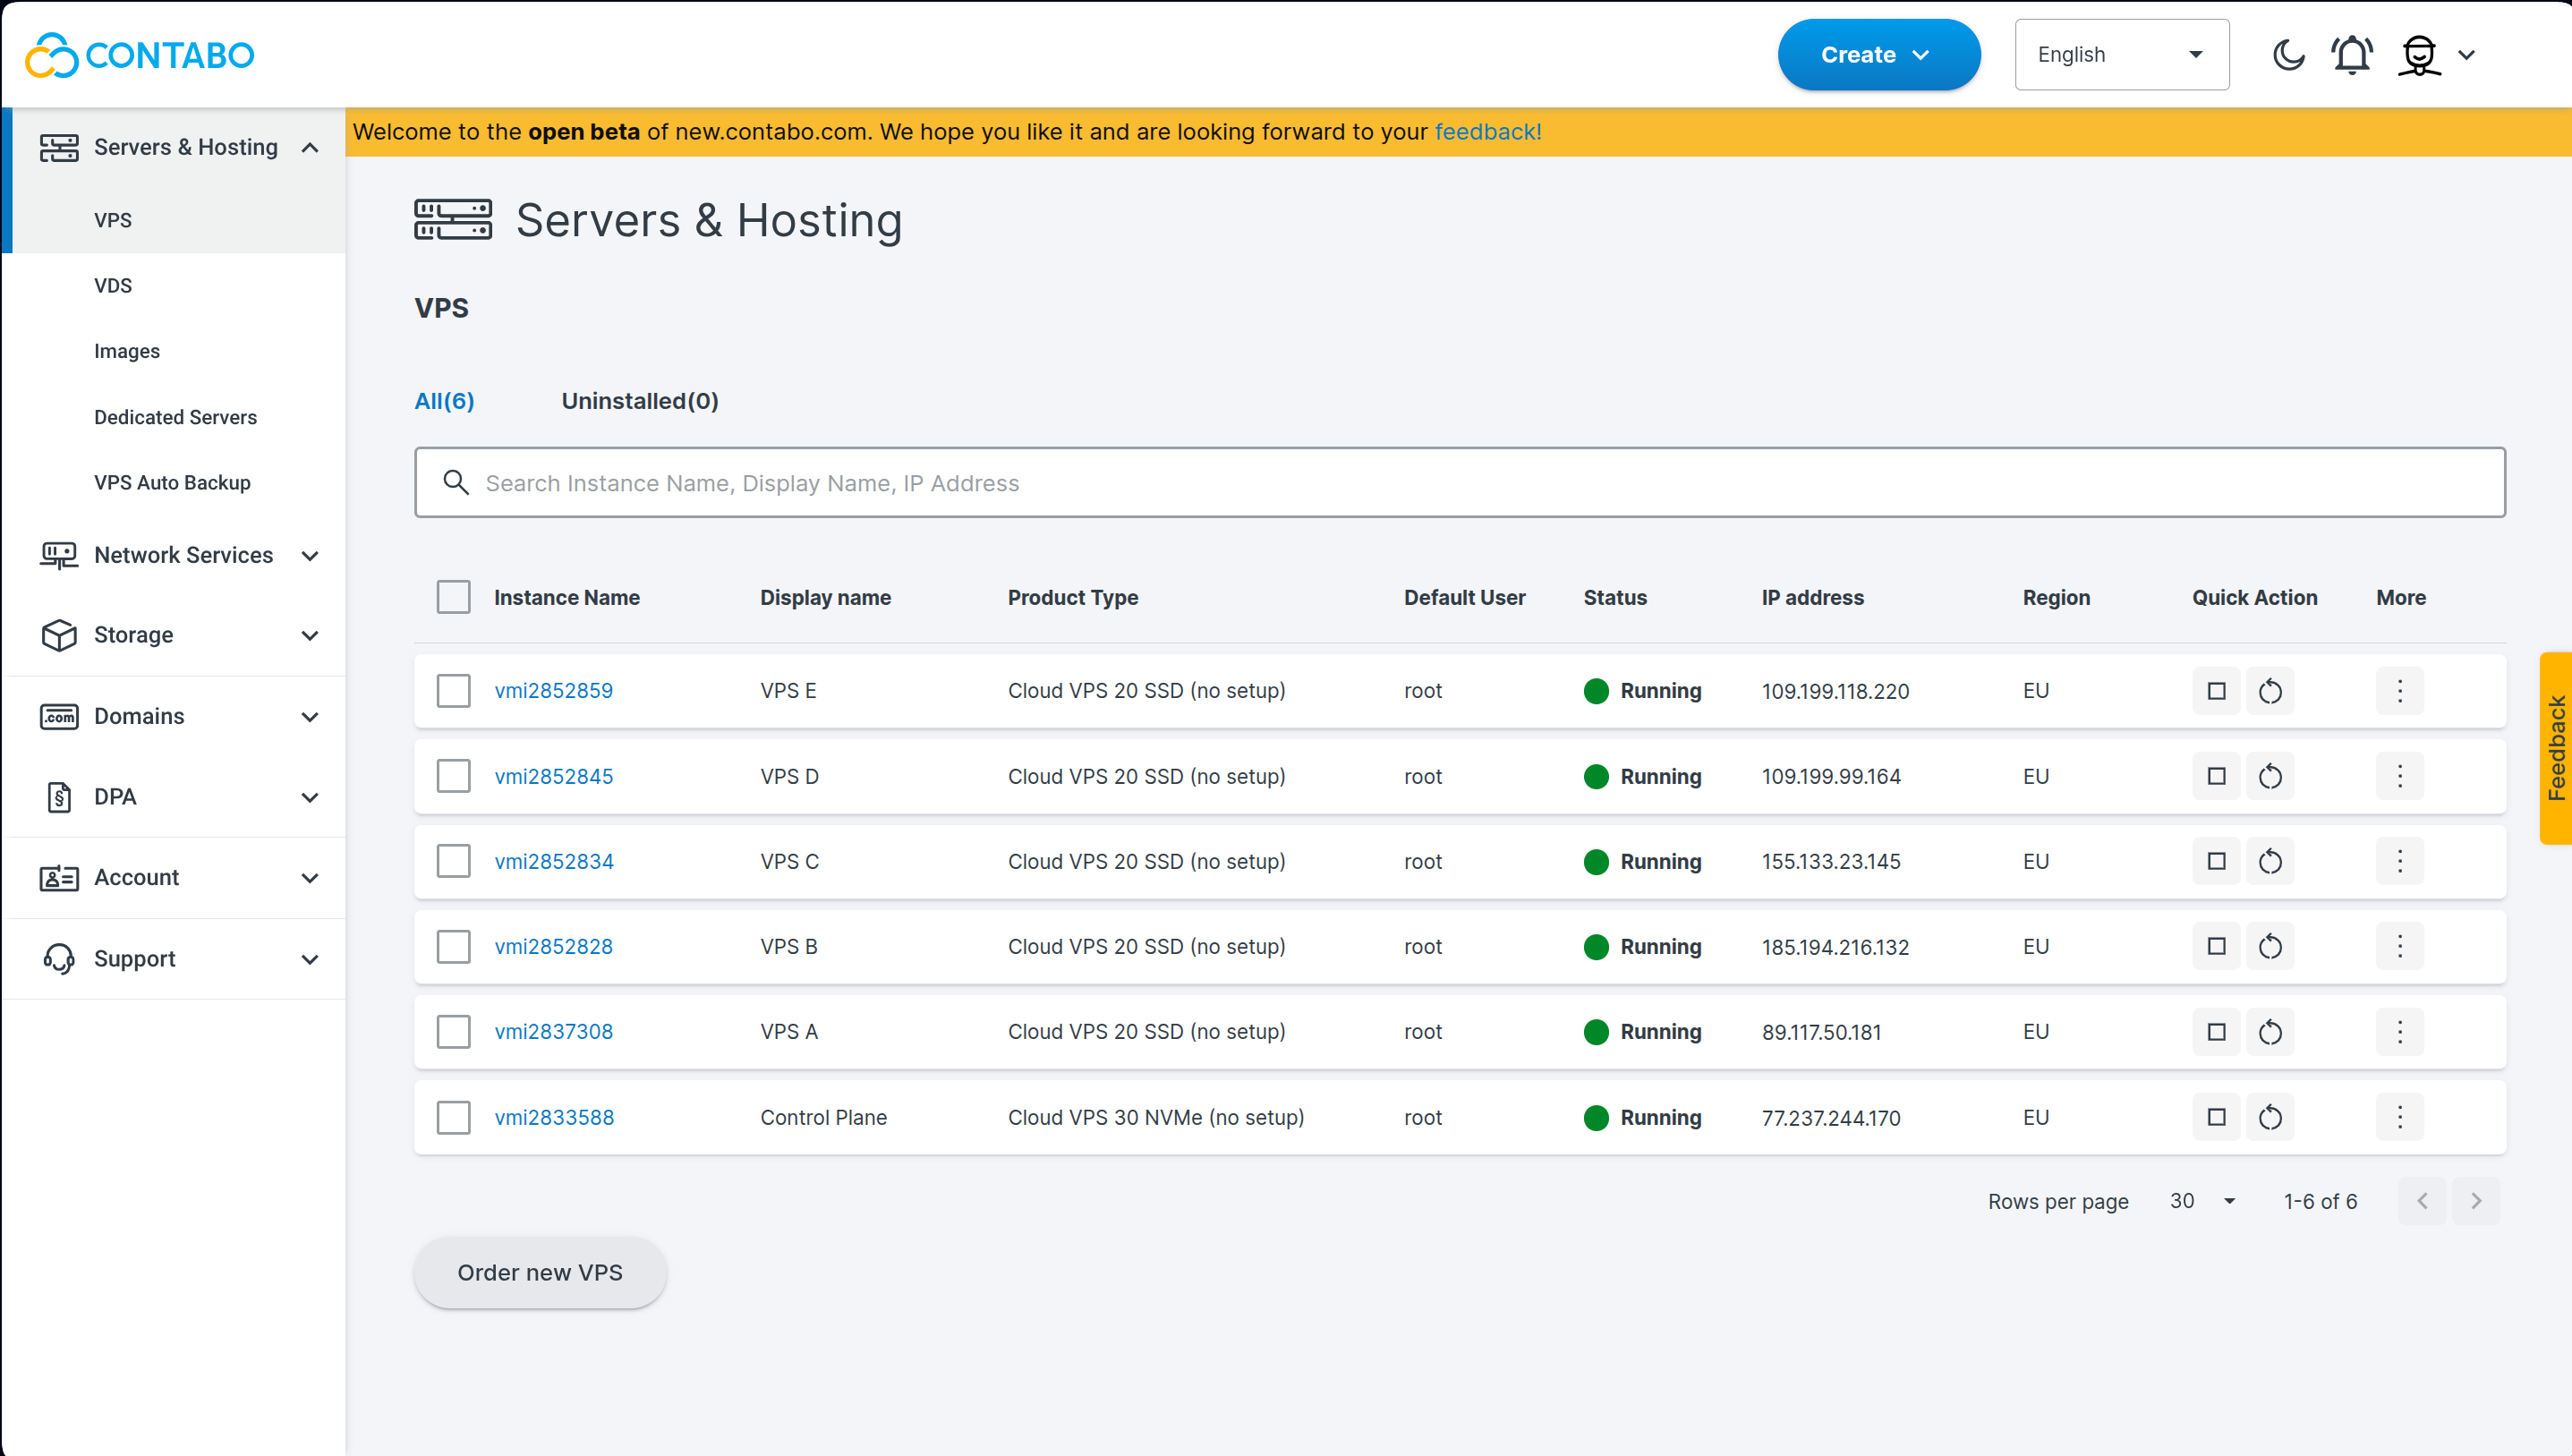
\includegraphics[width=1\textwidth]{images/vps-contabo.png}
    \caption{Daftar instance VPS Aktif di Provider Cloud (Contabo) yang terdiri dari 1 Control Plane dan 5 Worker Nodes.}
    \label{fig:vps_contabo}
\end{figure}

\begin{figure}[H]
    \centering
    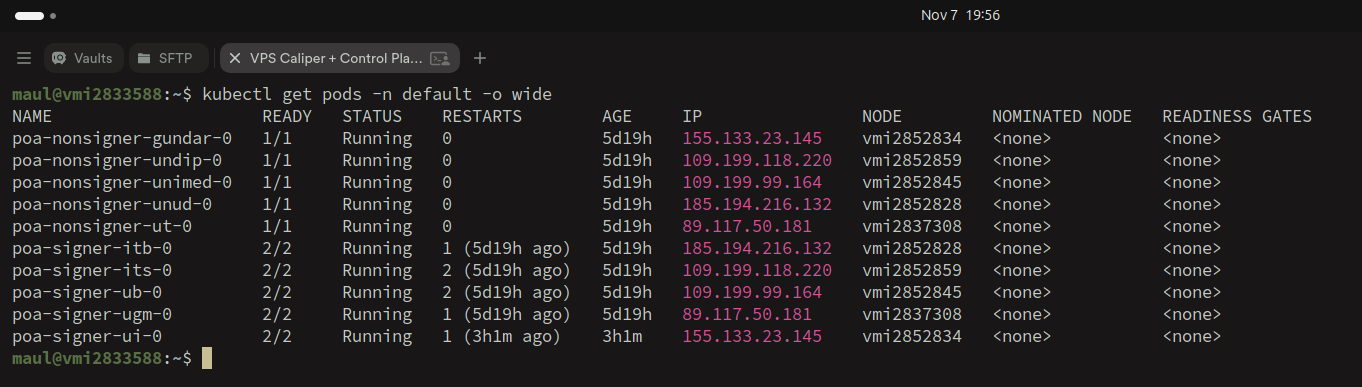
\includegraphics[width=1\textwidth]{images/kubectl-poa.png}
    \caption{Tampilan CLI \texttt{kubectl} yang menunjukkan status \textit{pods} container blockchain yang berjalan di dalam cluster Kubernetes.}
    \label{fig:kubectl_status}
\end{figure}

\clearpage
\subsection{Evolusi Topologi Jaringan (Ethstats)}
Dokumentasi ini menunjukkan perubahan topologi jaringan sesuai skenario pengujian (Skenario 1, 2, dan 3) yang dipantau melalui dashboard Ethstats.

\subsubsection{Proof of Authority (PoA)}
\begin{figure}[H]
    \centering
    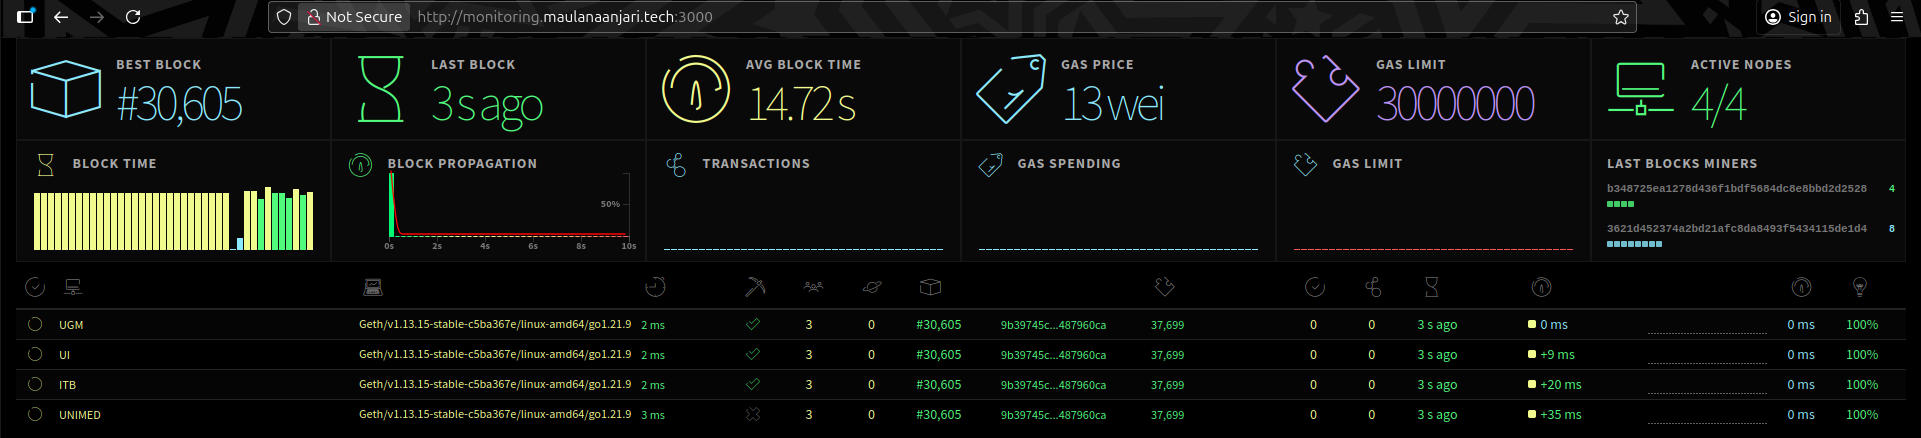
\includegraphics[width=1\textwidth]{images/ethstats-poa-3s-1ns.png}
    \caption{Ethstats PoA Skenario 1: 3 Signer + 1 Non-Signer (Total 4 Node).}
\end{figure}
\begin{figure}[H]
    \centering
    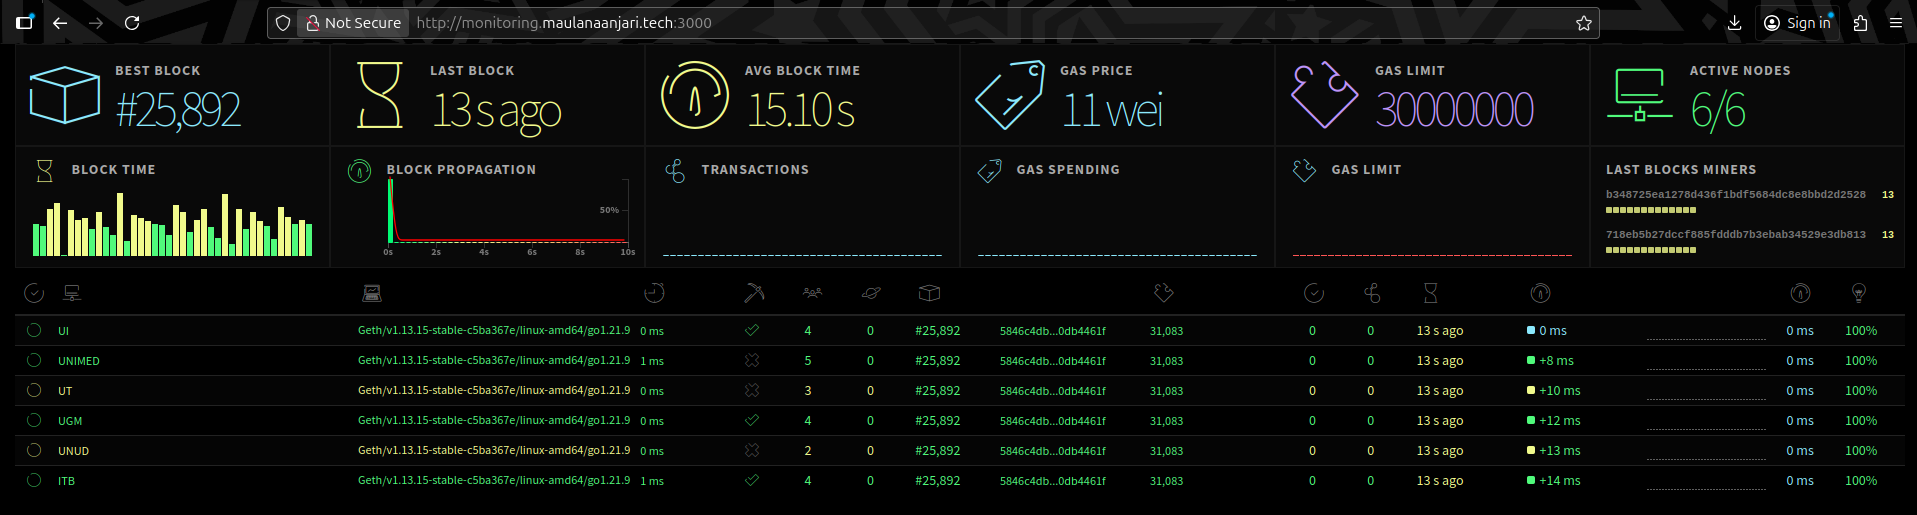
\includegraphics[width=1\textwidth]{images/ethstats-poa-3s-3ns.png}
    \caption{Ethstats PoA Skenario 2: 3 Signer + 3 Non-Signer (Total 6 Node).}
\end{figure}
\begin{figure}[H]
    \centering
    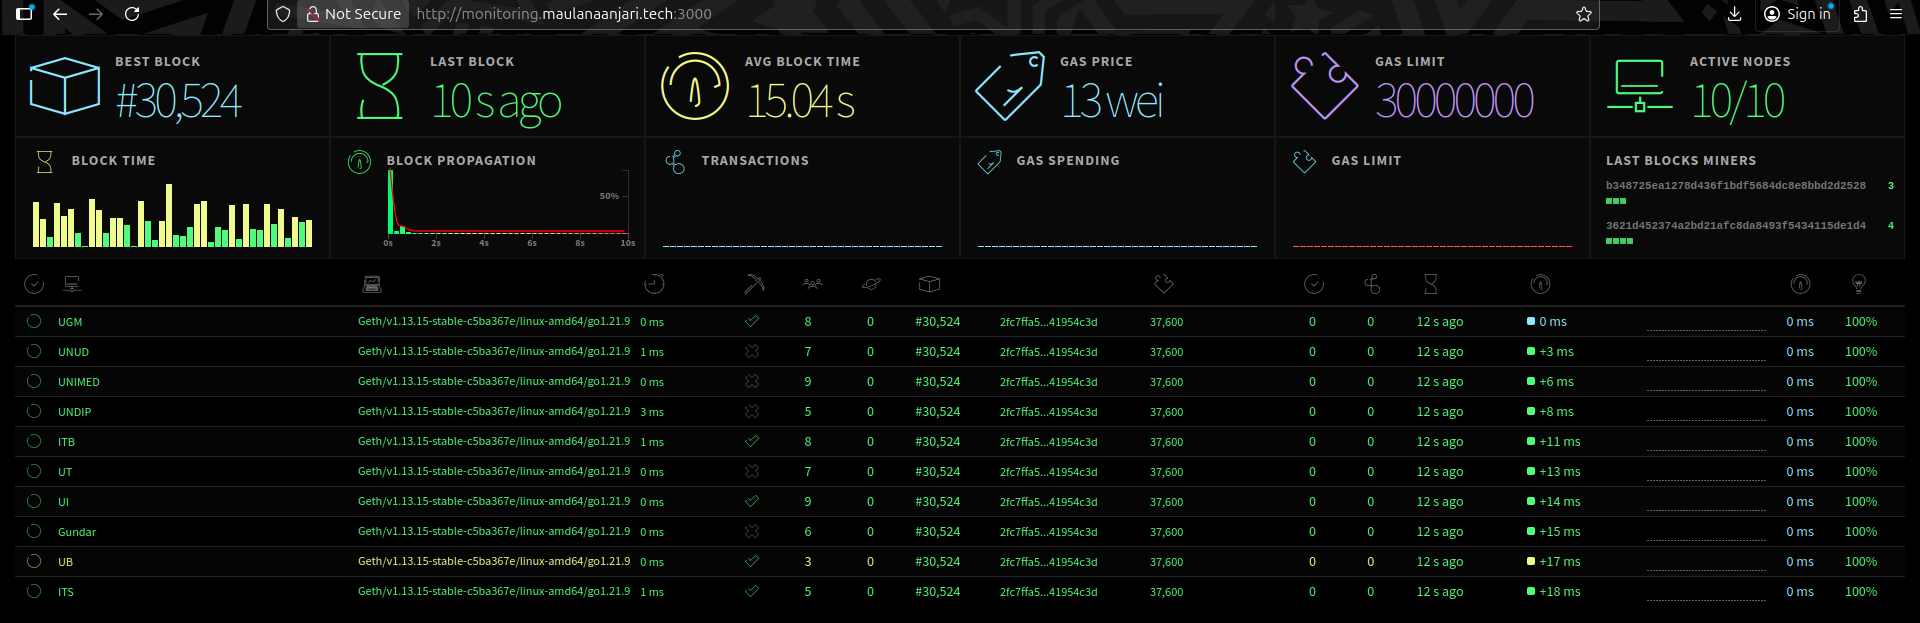
\includegraphics[width=1\textwidth]{images/ethstats-poa-5s-5ns.png}
    \caption{Ethstats PoA Skenario 3: 5 Signer + 5 Non-Signer (Total 10 Node).}
\end{figure}

\clearpage
\subsubsection{Proof of Stake (PoS)}
\begin{figure}[H]
    \centering
    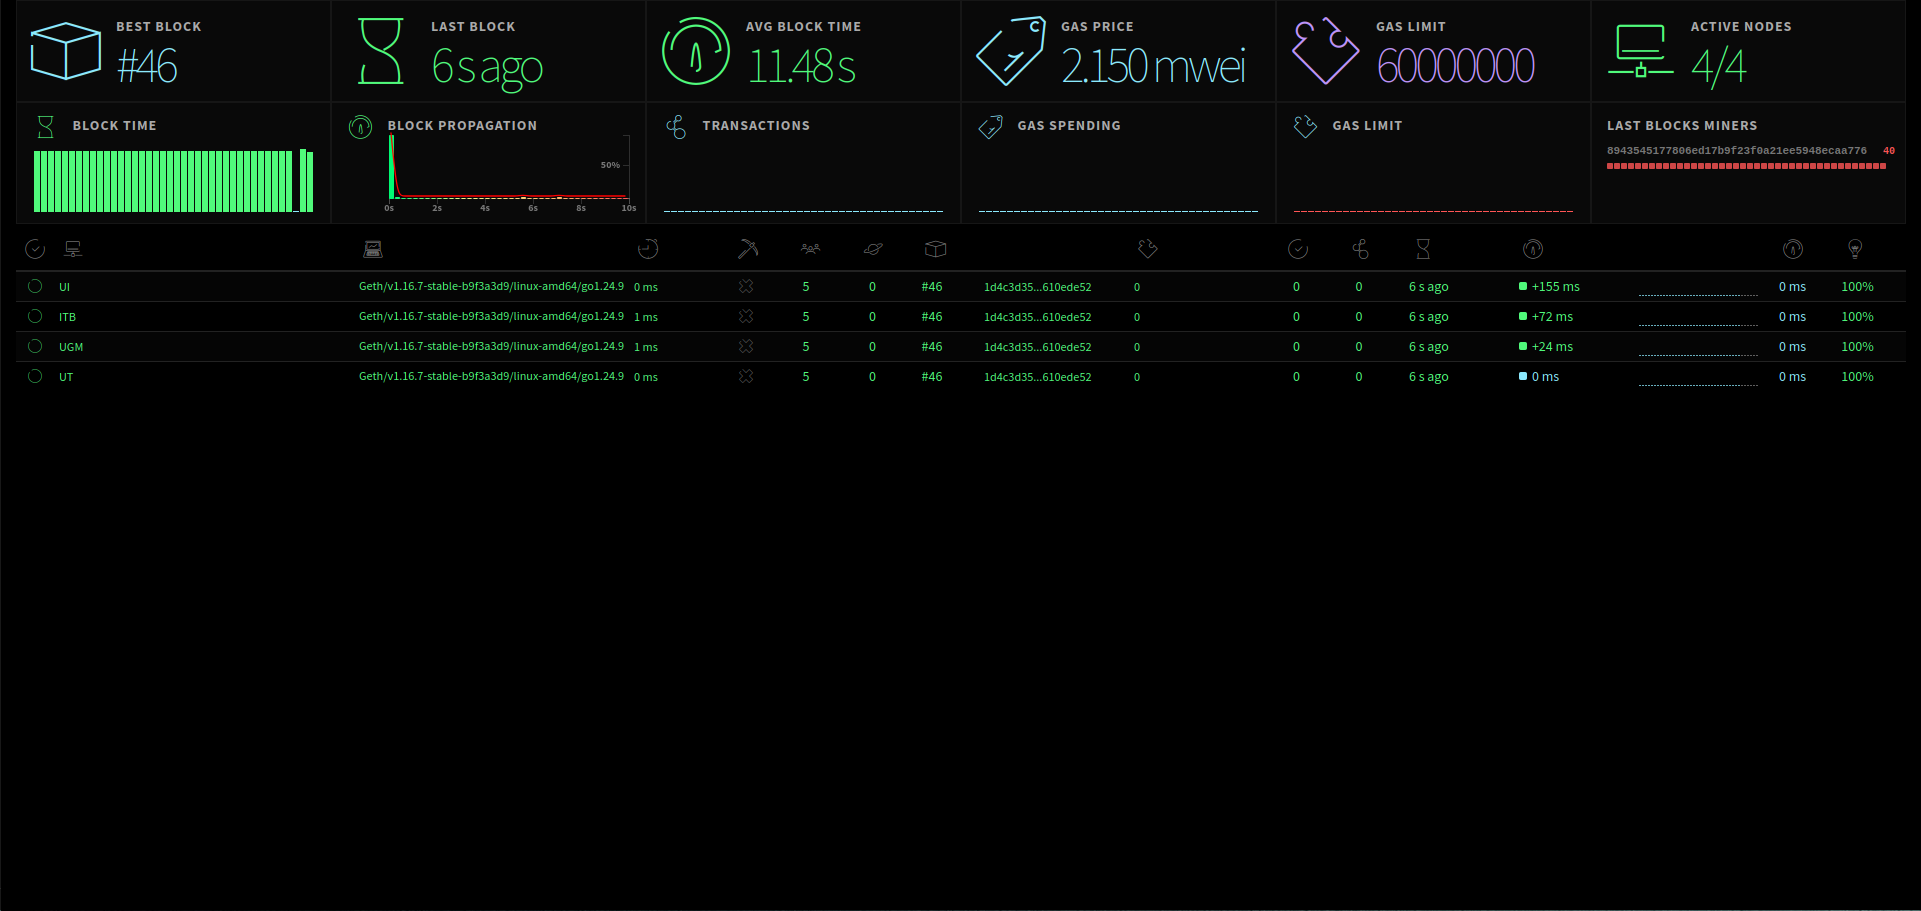
\includegraphics[width=1\textwidth]{images/ethstats-pos-3v-1nv.png}
    \caption{Ethstats PoS Skenario 1: 3 Validator + 1 Non-Validator (Total 4 Node).}
\end{figure}
\begin{figure}[H]
    \centering
    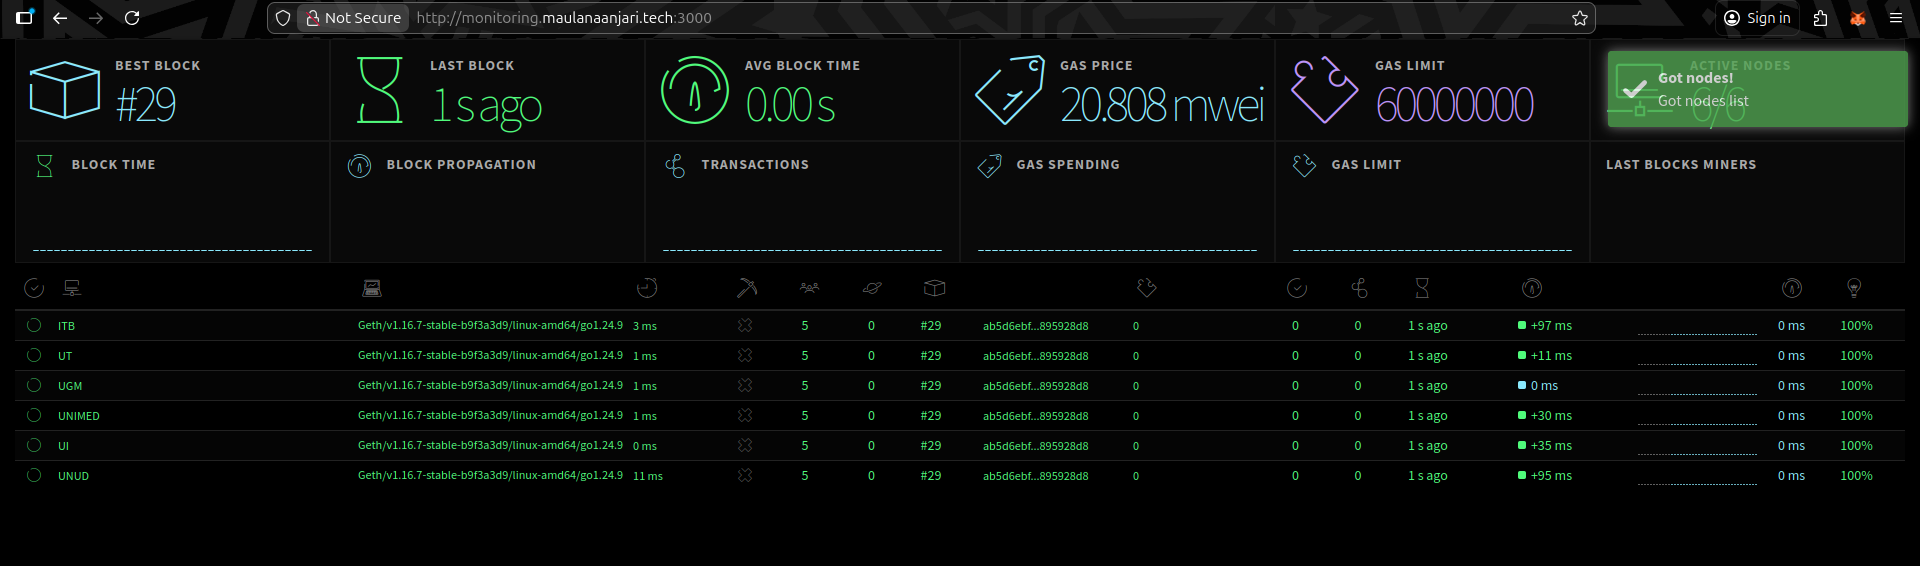
\includegraphics[width=1\textwidth]{images/ethstats-pos-3v-3nv.png}
    \caption{Ethstats PoS Skenario 2: 3 Validator + 3 Non-Validator (Total 6 Node).}
\end{figure}
\begin{figure}[H]
    \centering
    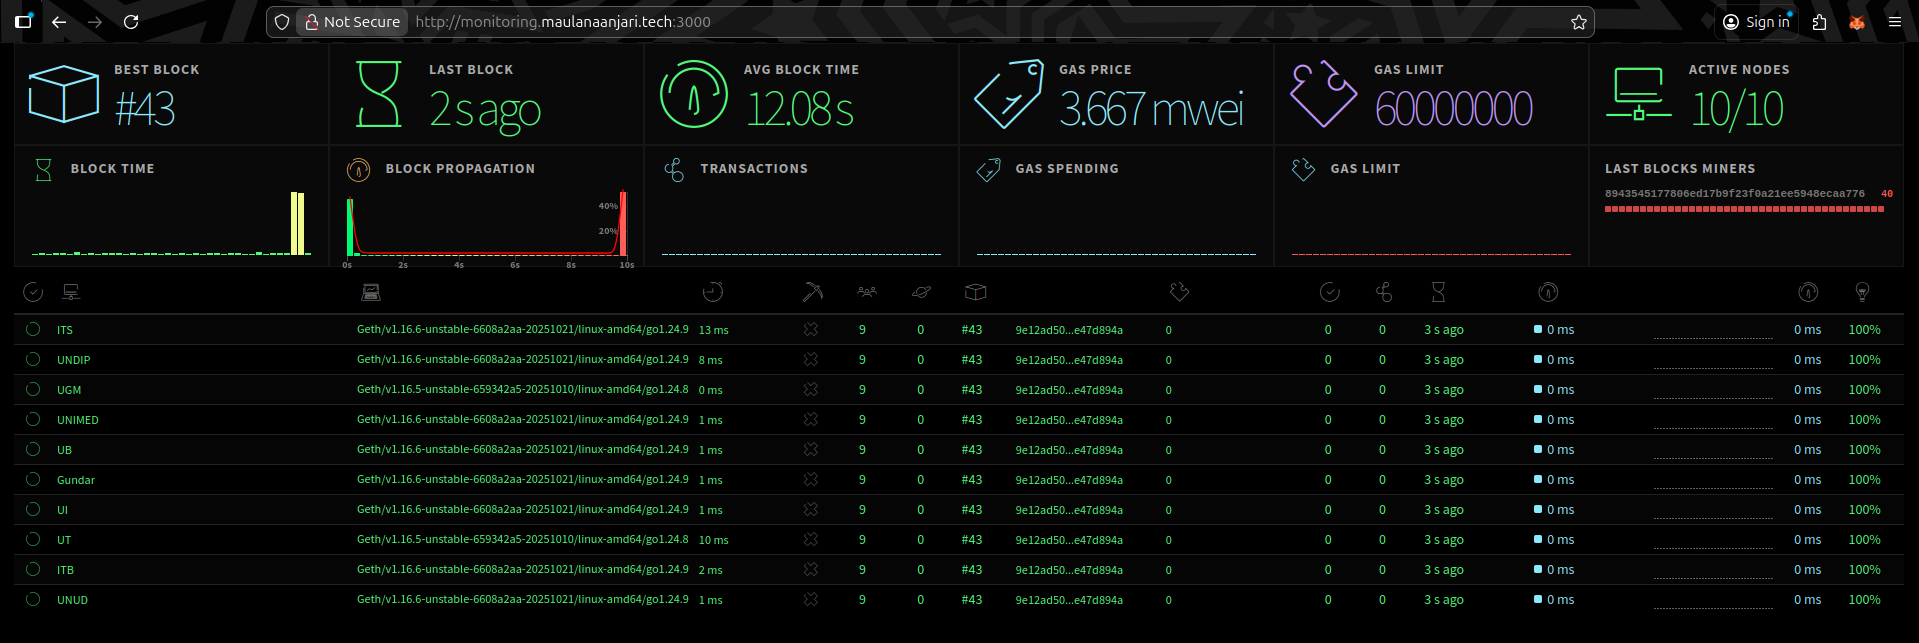
\includegraphics[width=1\textwidth]{images/ethstats-pos-5v-5nv.png}
    \caption{Ethstats PoS Skenario 3: 5 Validator + 5 Non-Validator (Total 10 Node).}
\end{figure}

\clearpage
\subsection{Status Konektivitas Monitoring (Prometheus)}
Halaman \textit{Targets} pada Prometheus yang memverifikasi bahwa seluruh \textit{exporter} data (Node Exporter, cAdvisor, Geth) terhubung dengan sukses (State: UP).

\begin{figure}[H]
    \centering
    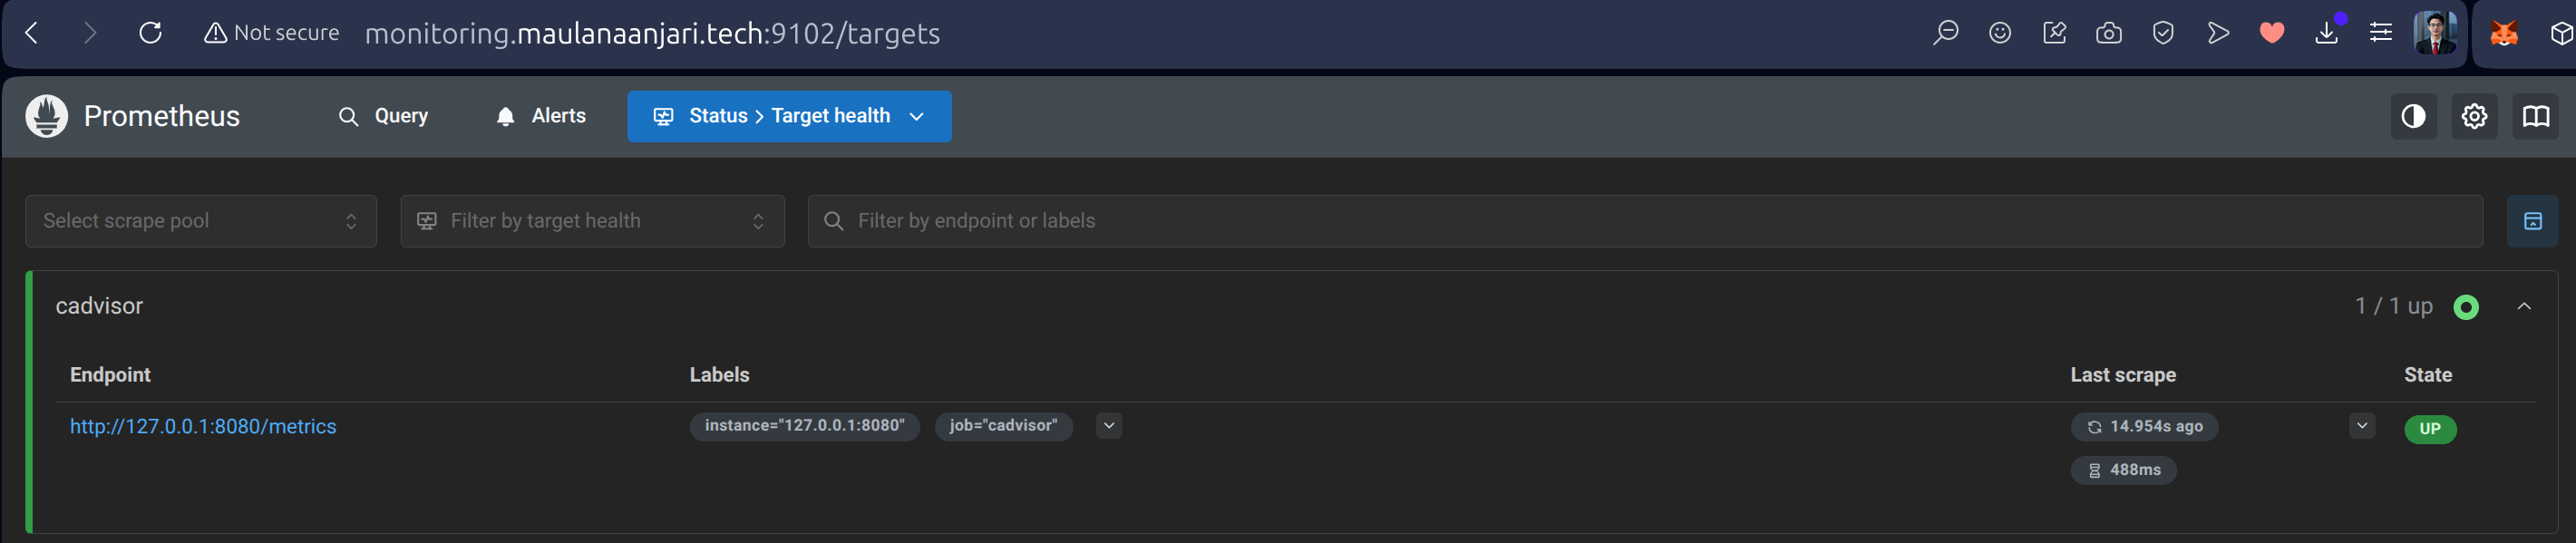
\includegraphics[width=1\textwidth]{images/prometheus-poa-all-connected-1.png}
    \caption{Status Target Prometheus (Bagian 1): Koneksi ke cAdvisor Container.}
\end{figure}
\begin{figure}[H]
    \centering
    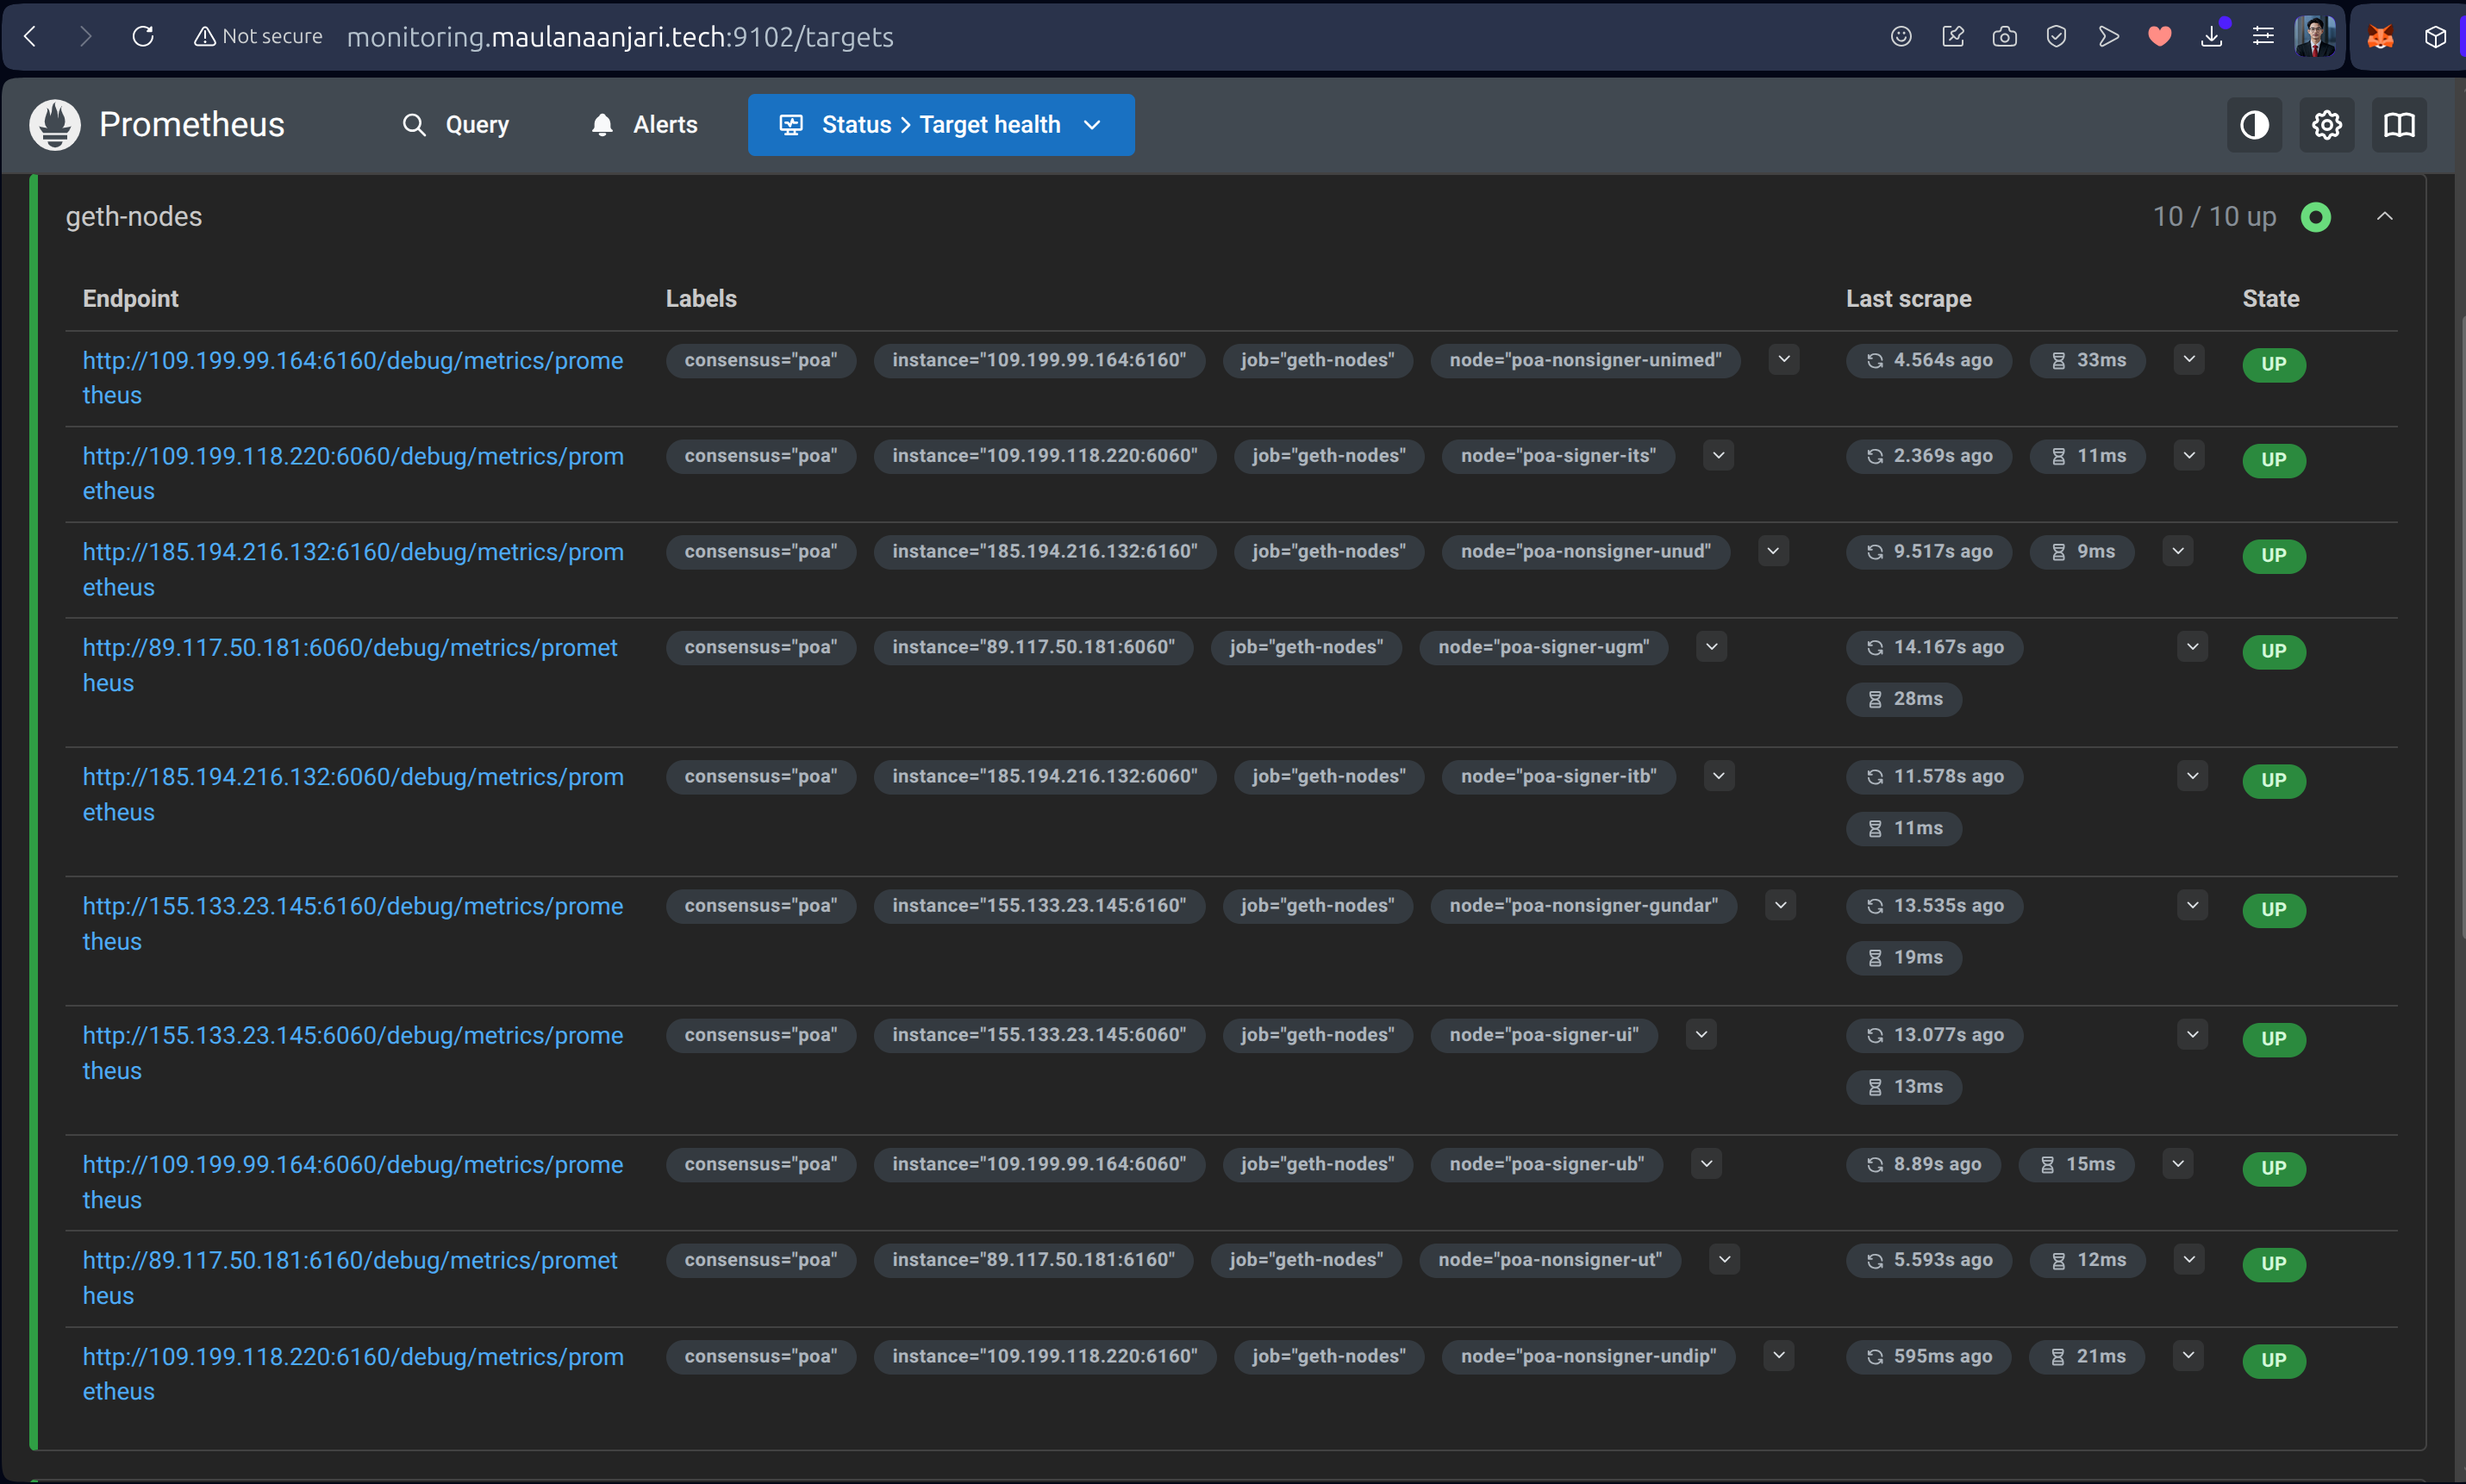
\includegraphics[width=1\textwidth]{images/prometheus-poa-all-connected-2.png}
    \caption{Status Target Prometheus (Bagian 2): Koneksi ke Geth Metrics.}
\end{figure}
\begin{figure}[H]
    \centering
    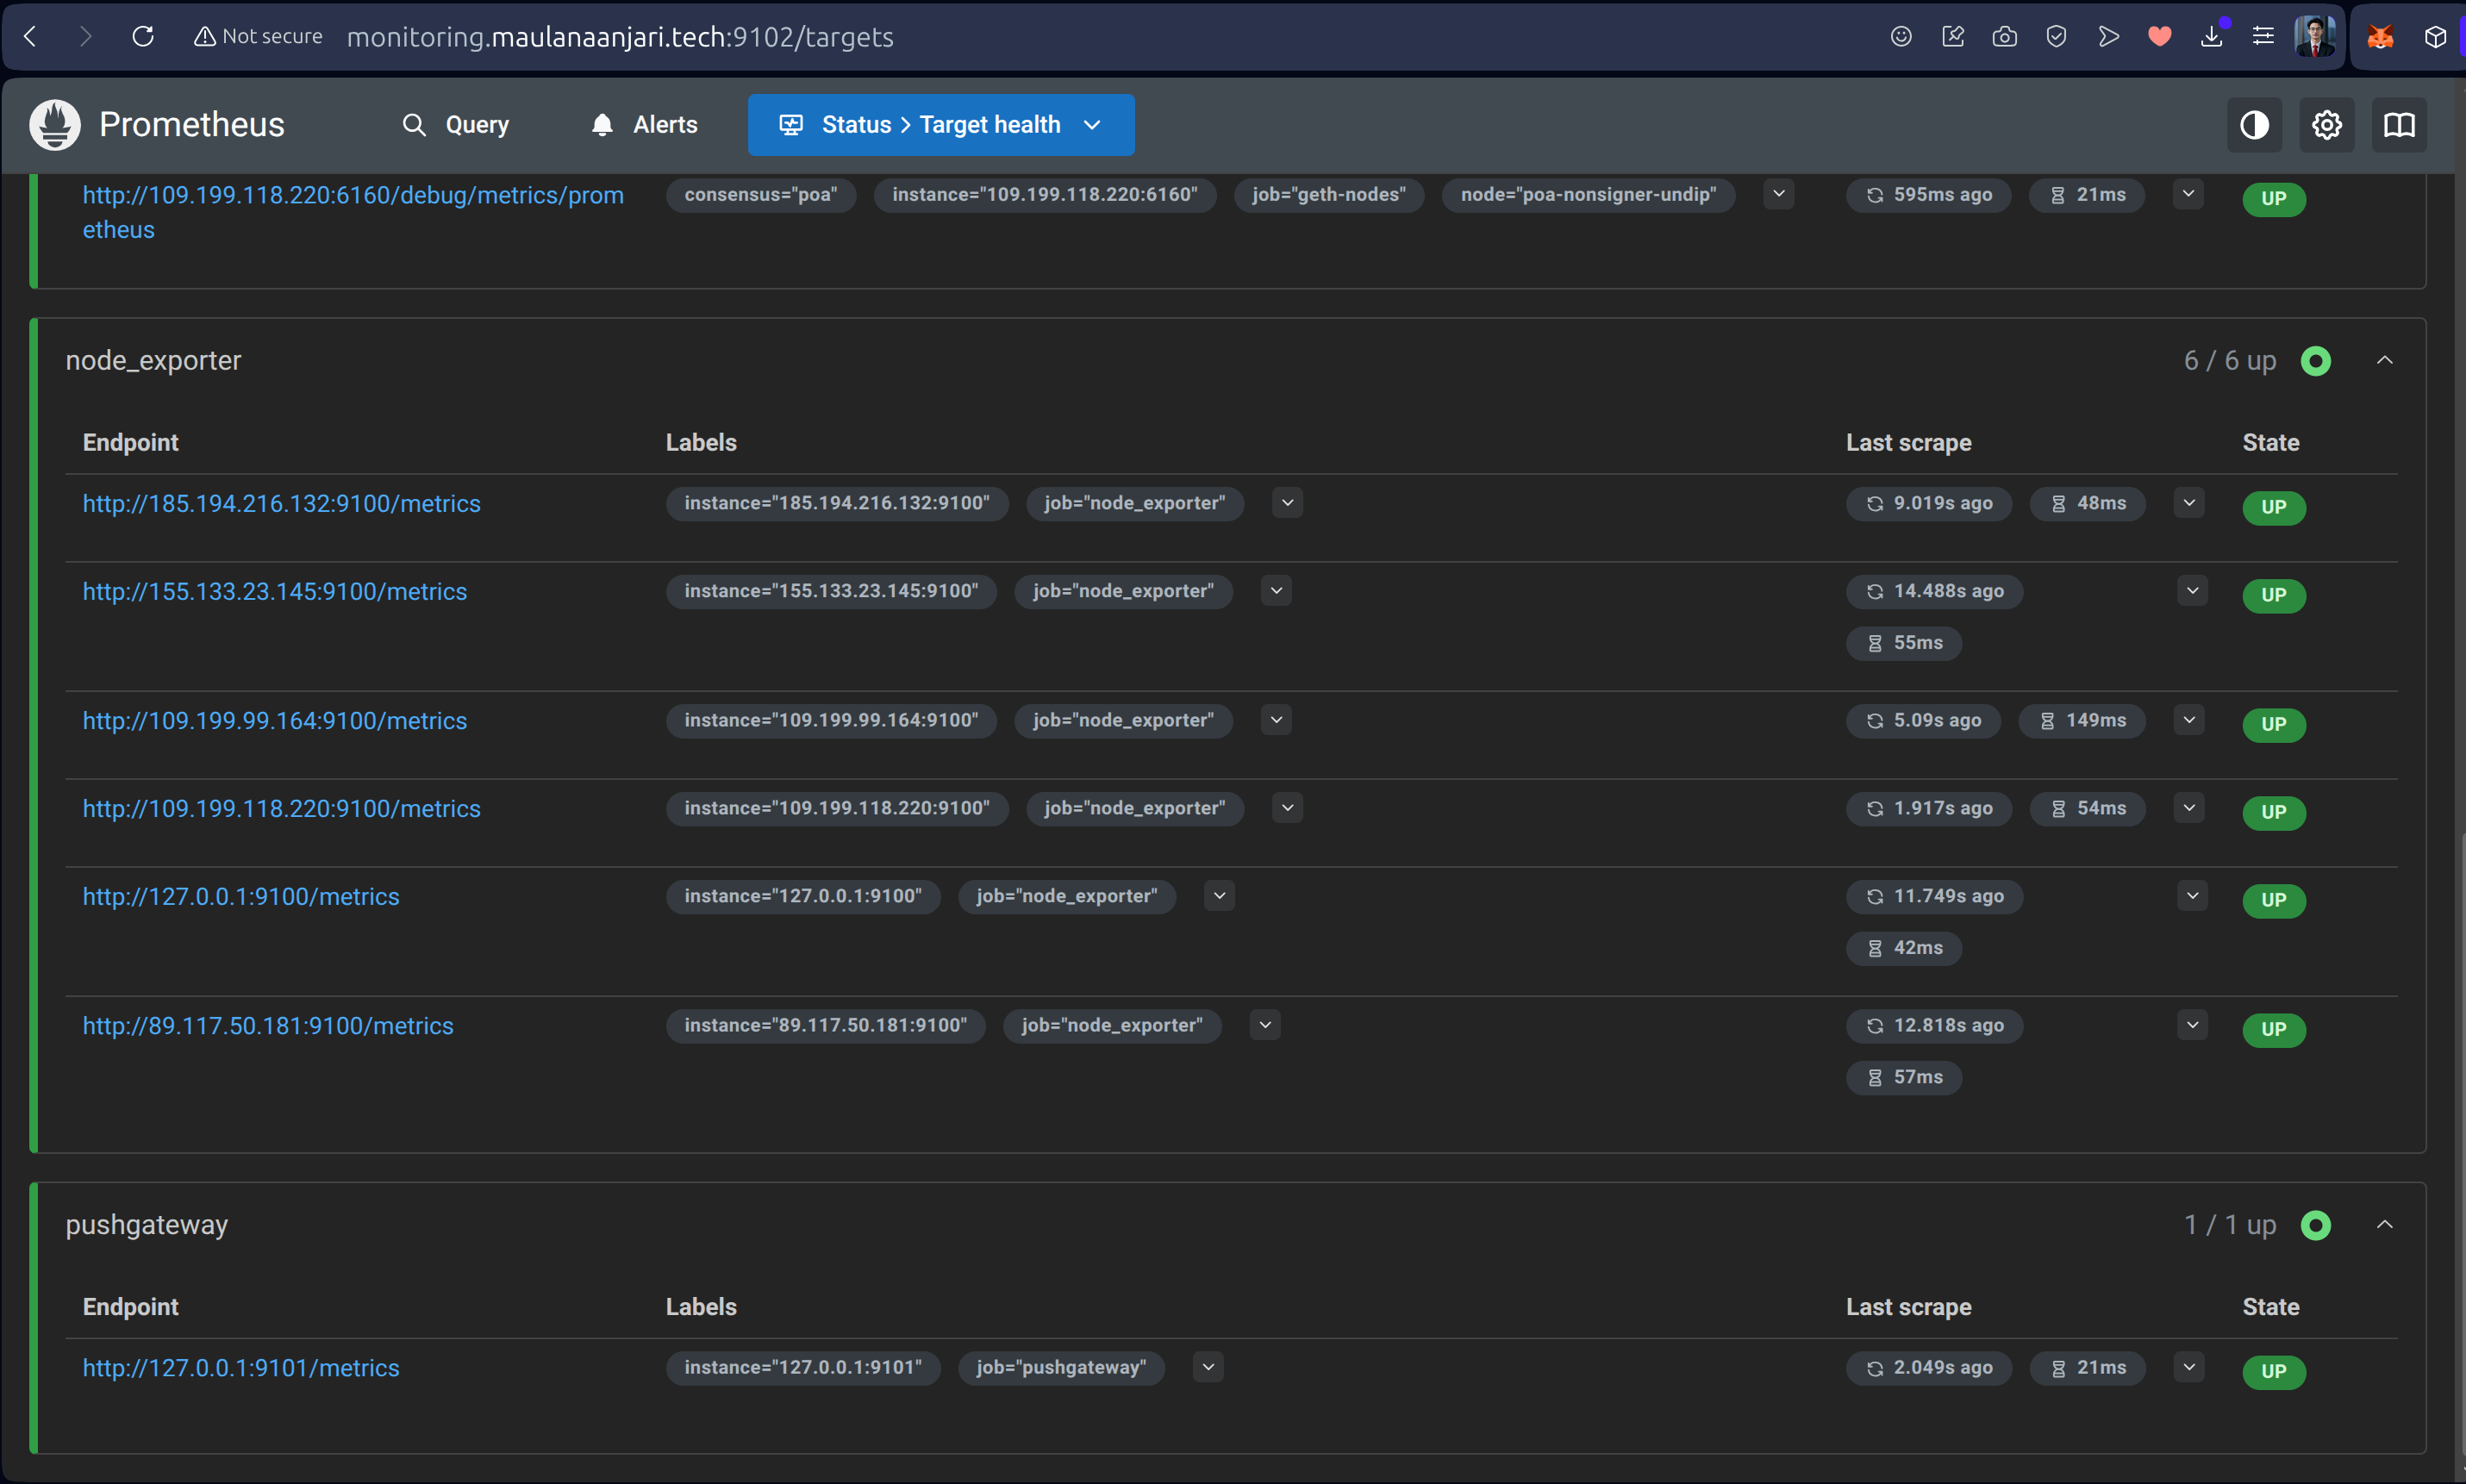
\includegraphics[width=1\textwidth]{images/prometheus-poa-all-connected-3.png}
    \caption{Status Target Prometheus (Bagian 3): Koneksi ke Node Exporter dan Pushgateway.}
\end{figure}

\clearpage
\subsection{Visualisasi Beban Sistem (Grafana)}
\begin{figure}[H]
    \centering
    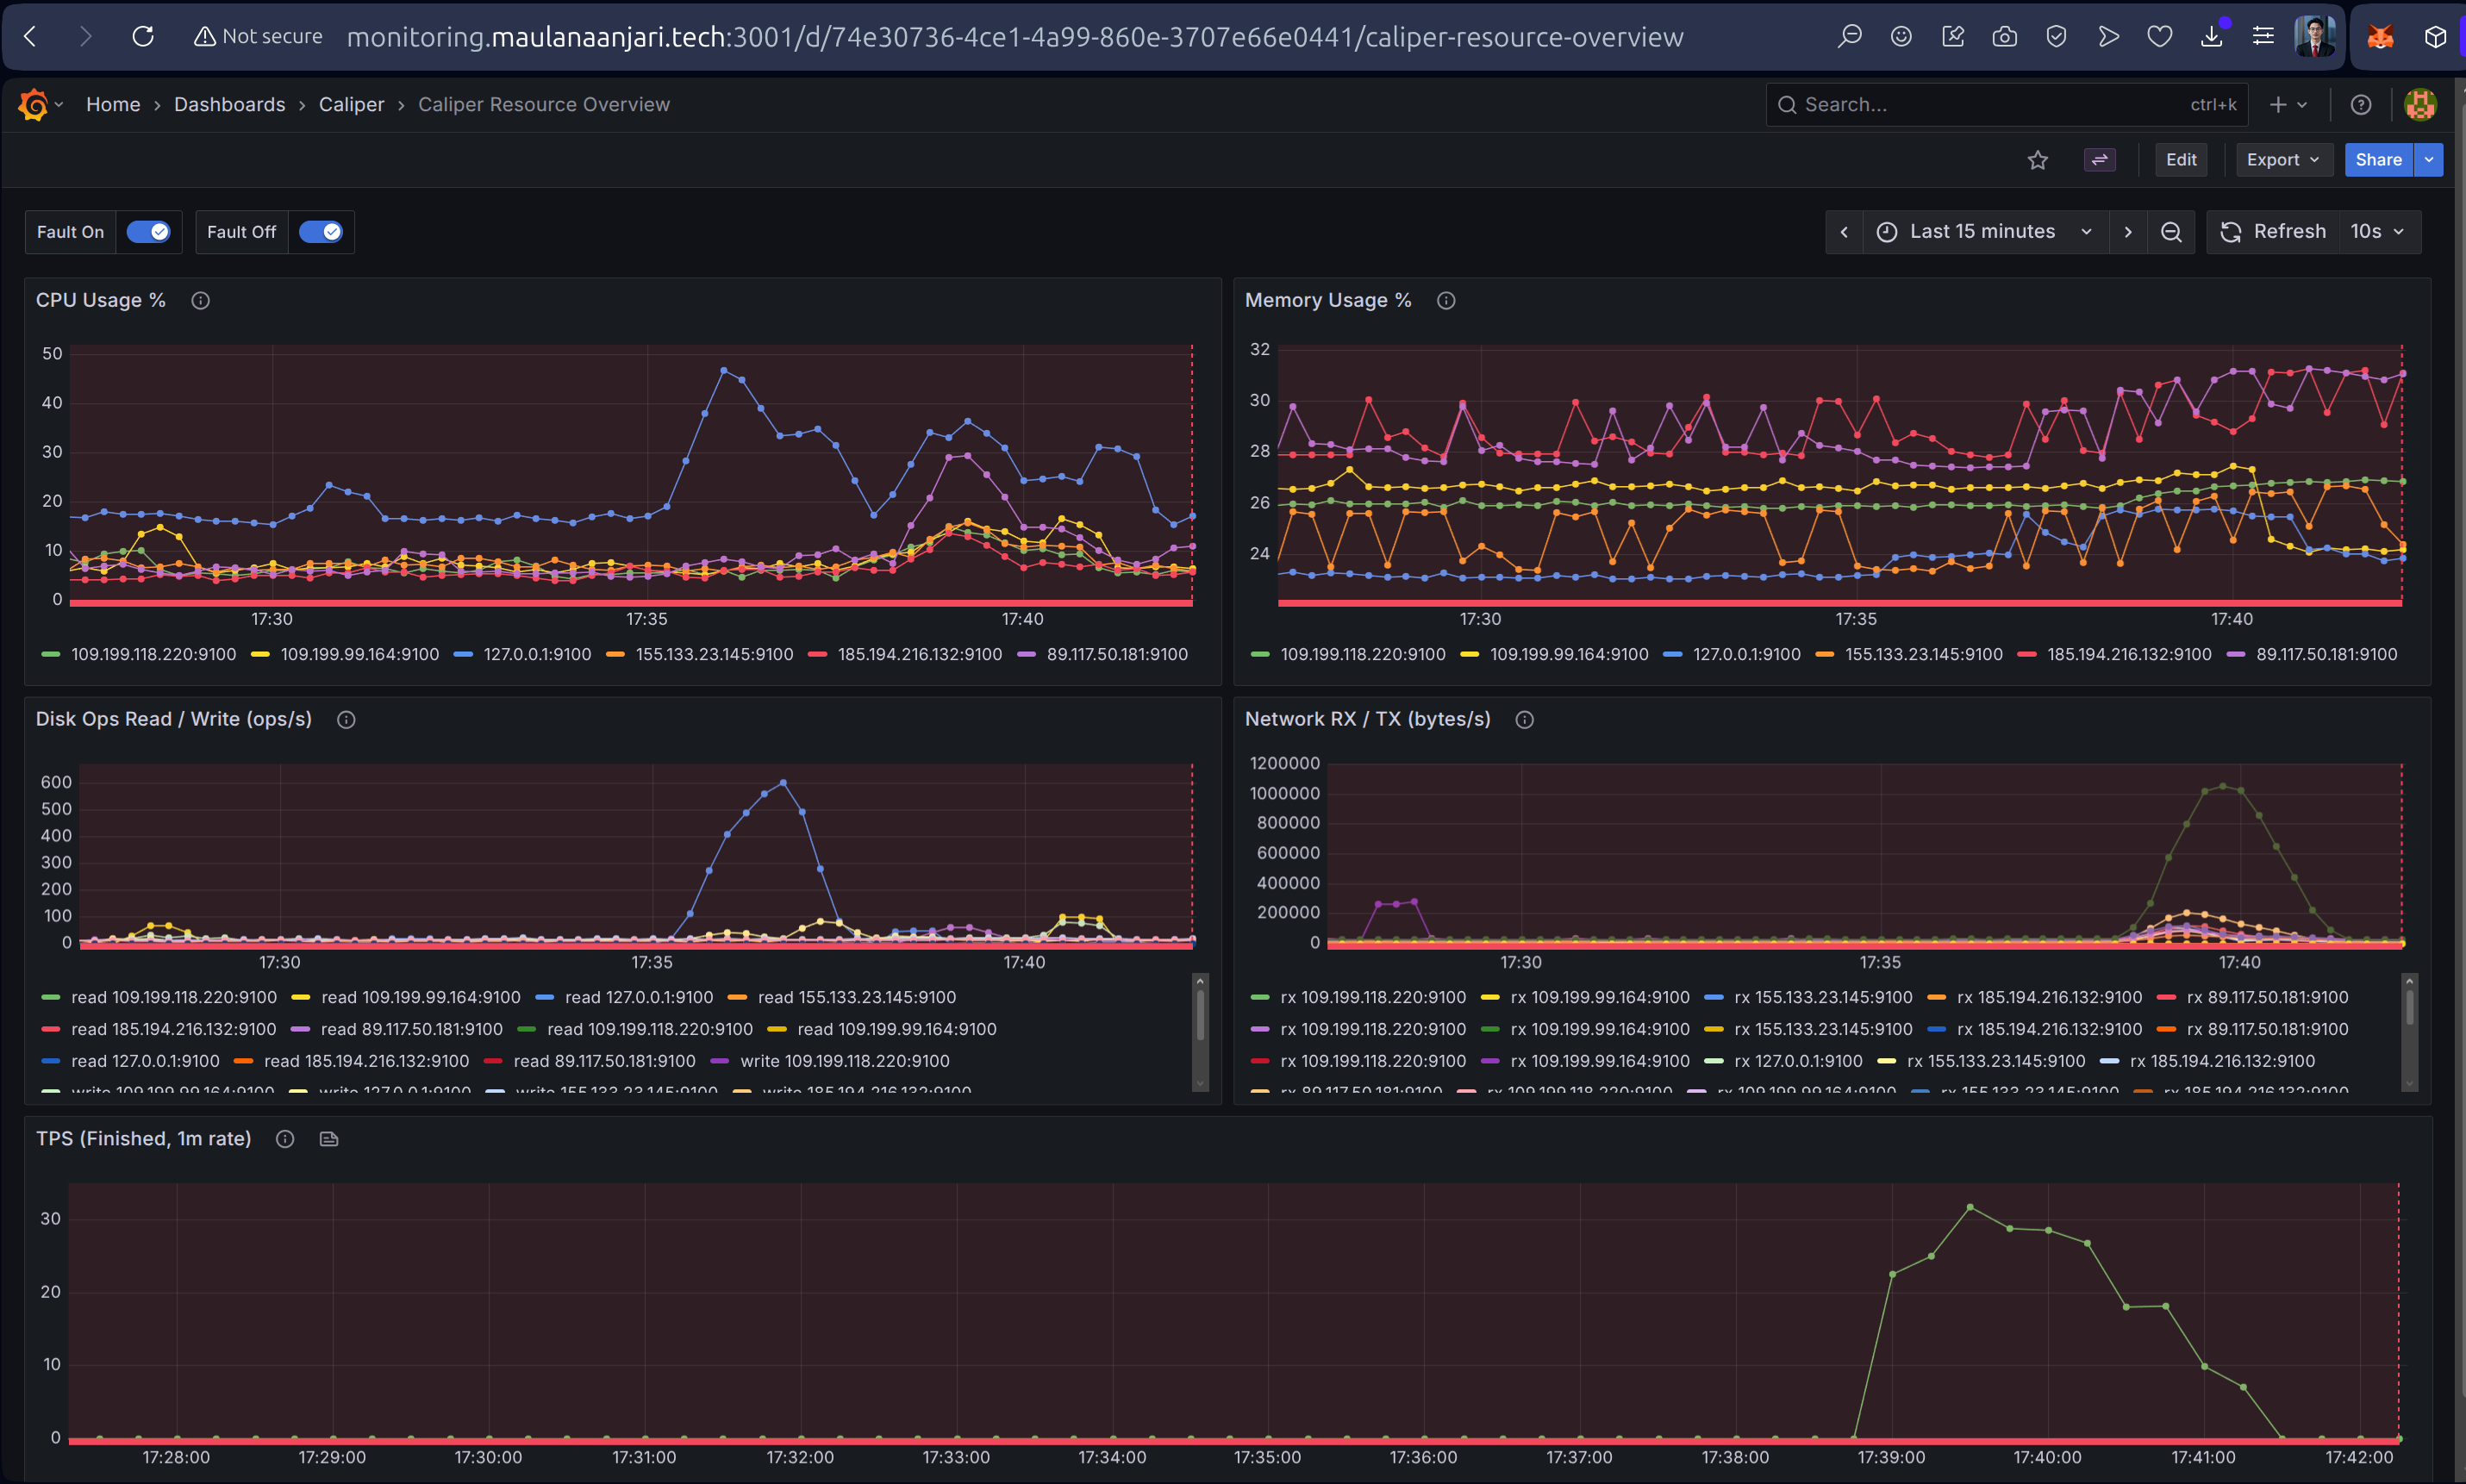
\includegraphics[width=1\textwidth]{images/grafana_resource_spike.png}
    \caption{Dashboard Grafana saat \textit{Load Test} 70 TPS. Terlihat korelasi antara panel TPS (bawah) yang aktif dengan lonjakan penggunaan CPU (kiri atas) dan Network (kanan tengah) pada seluruh node.}
    \label{fig:grafana_spike_full}
\end{figure}
